\documentclass[12px]{article}

\title{Lezione 31 Geometria I}
\date{2024-05-22}
\author{Federico De Sisti}

\usepackage{amsmath}
\usepackage{amsthm}
\usepackage{mdframed}
\usepackage{amssymb}
\usepackage{nicematrix}
\usepackage{amsfonts}
\usepackage{tcolorbox}
\tcbuselibrary{theorems}
\usepackage{xcolor}
\usepackage{cancel}

\newtheoremstyle{break}
  {1px}{1px}%
  {\itshape}{}%
  {\bfseries}{}%
  {\newline}{}%
\theoremstyle{break}
\newtheorem{theo}{Teorema}
\theoremstyle{break}
\newtheorem{lemma}{Lemma}
\theoremstyle{break}
\newtheorem{defin}{Definizione}
\theoremstyle{break}
\newtheorem{propo}{Proposizione}
\theoremstyle{break}
\newtheorem*{dimo}{Dimostrazione}
\theoremstyle{break}
\newtheorem*{es}{Esempio}

\newenvironment{dimo}
  {\begin{dimostrazione}}
  {\hfill\square\end{dimostrazione}}

\newenvironment{teo}
{\begin{mdframed}[linecolor=red, backgroundcolor=red!10]\begin{theo}}
  {\end{theo}\end{mdframed}}

\newenvironment{nome}
{\begin{mdframed}[linecolor=green, backgroundcolor=green!10]\begin{nomen}}
  {\end{nomen}\end{mdframed}}

\newenvironment{prop}
{\begin{mdframed}[linecolor=red, backgroundcolor=red!10]\begin{propo}}
  {\end{propo}\end{mdframed}}

\newenvironment{defi}
{\begin{mdframed}[linecolor=orange, backgroundcolor=orange!10]\begin{defin}}
  {\end{defin}\end{mdframed}}

\newenvironment{lemm}
{\begin{mdframed}[linecolor=red, backgroundcolor=red!10]\begin{lemma}}
  {\end{lemma}\end{mdframed}}

\newcommand{\icol}[1]{% inline column vector
  \left(\begin{smallmatrix}#1\end{smallmatrix}\right)%
}

\newcommand{\irow}[1]{% inline row vector
  \begin{smallmatrix}(#1)\end{smallmatrix}%
}

\newcommand{\matrice}[1]{% inline column vector
  \begin{pmatrix}#1\end{pmatrix}%
}

\newcommand{\C}{\mathbb{C}}
\newcommand{\K}{\mathbb{K}}
\newcommand{\R}{\mathbb{R}}


\begin{document}
	\maketitle
	\newpage
	\section{Due Teoremi Classici}
	\begin{teo}[Desgardes]
		$\pro =\pro(V)$ piano proiettivo, $P_1,\ldots,P_6\in\pro$ punti distinti tali che le tre rette
		\[
		 L(P_1,P_4) \ \ L(P_2,P_4) \ \ L(P_3,P_6)
		.\] 
		abbiano in comune un punto $P_0\neq P_i \ \ 1\leq i \leq 6$
	Allora
	\[
	L(P_1,P_3)\cap L(P_4,P_6),L(P_2,P_5)\cap L(P_5,P_6),L(P_1,P_2)\cap L(P_4,P_5)
	.\] 
	sono allineati
	\end{teo}
	\begin{dimo}\ 
		\begin{center}
			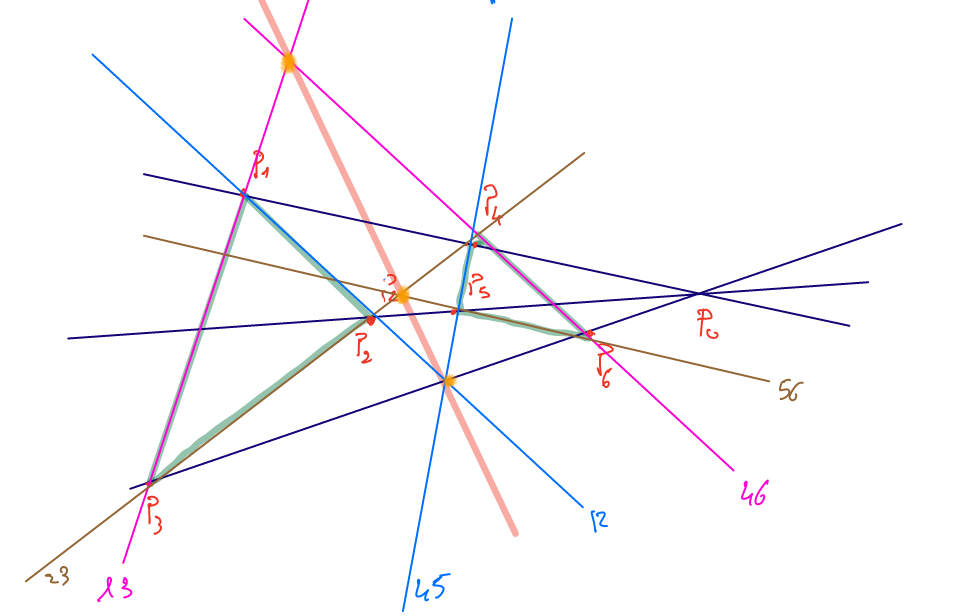
\includegraphics[scale=.35]{Desargues.png}
		\end{center}
	Siano $v_i\in V, \ \0\leq i \leq 6, $ t.c. $\ \ [v_i] = P_i$ Per ipotesi
	\[
	v_0 = \alpha_1v_1+\alpha_4v_4 = \alpha_2v_2+\alpha_5v_5=\alpha_3v_3+\alpha_6v_6
	.\] 
	Inoltre poiché $P_0\neq P_i, i > 1 ,$ tutti gli $\alpha_i$ sono non nulli.
	I punti \\
	\begin{aligend}
		&L(P_1,P_3)\cap L(P_4,P_6)\\
		&L(P_2,P_3)\cap L(P_5,P_6)\\
		&L(P_1,P_2)\cap L(P_4,P_5)
	\end{aligend} sono associati ai vettori \\
	\begin{aligend}		
&\alpha_1v_1-\alpha_3v_3=-\alpha_4v_4+\alpha_6v_6\\
&-\alpha_2v_2 + \alpha_3v_3=\alpha_5v_4-\alpha_6v_6 \\
&- \alpha_1v_1+\alpha_2v_2=\alpha_4v_4-\alpha_5v_5
		\end{aligend}\\
		I vettori nella colonna di sinistra sono dipendenti, poiché la loro somma è 0. Dunque i punti corrispondenti sono allineati.
	\end{dimo}
	\begin{teo}[Pappo]
	$A_1,\ldots,A_6$ distinti $L(A_1,A_2),L(A_2,A_3),\ldots,L(A_6,A_1)$ distinte\\
	esistono $r,s$ rette con $A_i\in r$, i dispari, $A_i\in s$ i pari\\
	Supponiamo poi $0=r\cap s\neq A_i.$ Allora 
	\[
	L(A_1,A_2)\cap L(A_4,A_5), \ \ L(A_2,A_3)\cap L(A_5,A_6),\ \ L(A_3,A_4)\cap L(A_6,A_1)
	.\] 
	sono allineati
\end{teo}
\begin{center}
	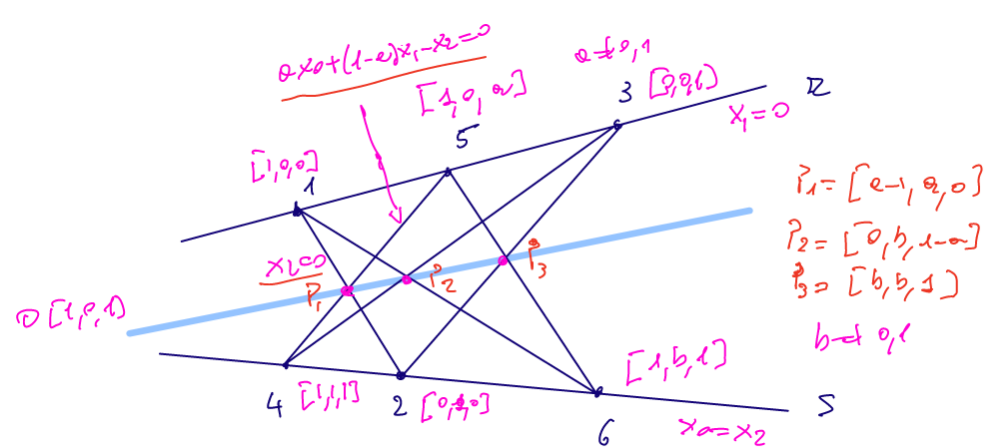
\includegraphics[scale=.45]{Pappo.png}
\end{center}
\begin{dimo}
	Poiché $r = L(A_1,A_3),\ \ s=L(A_2,A_4)$ sono distati e $0\neq A_i$\\
	$A_1,A_2,A_3,A_4$ è un riferimento proiettivo. Ma
	\[
		\det\matrice{a-1 & a & 0 \\ 0 &b &1 - a\\ b & b & 1} = 0 \Rightarrow  (a-1)b(1-1+a)+ab(1-a)=0
	\] 

\end{dimo}

\ \\ \hline \ \\
 $\pro=\pro(V)$ spazio proiettivo di dimensione $n$ $S = \pro (U),\ \ \ H = \pro(W)$ sottospazi proiettivi tali che 
 \[
  S\cap H = \emptyset \ \ \text{ e} \ \ \ L(S,H)=\pro
 .\] 
 Se $\dim S = k, \dim H = h$ per le formule di Grassmann
  \[
 k + h = n-1
 .\] 
$\forall P\in \pro\setminus H, \ \ \ \dim L(H,\{p\})=h+1$\\
Quindi $S\cap L(H,\{0\}) $ è un punto\\
Posso definire la proiezione su  $S$ di centro $H$ come
\[
 \pi^H_S: \pro\setminus H \rightarrow \pro
.\] 
\[
	P \rightarrow S\cap L(H,\{0\})
.\] 
$\pi^H_S$ è unna trasformazione proiettiva degenere indotta da $\pro^W_U :V \rightarrow V$ proiezione su $U$ parallela ad $H$\\
\begin{center}
	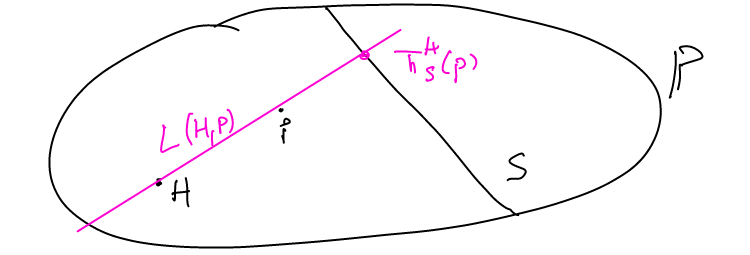
\includegraphics[scale=.45]{trasformazione_proiettiva.png}
\end{center}
 \section{Proiettività}
 Siano in $\pro^2\ \ r,s$ rette distinte con $A = r\cap s$
  \begin{defi}
 	Dato $O\not\in r\cup s,$ la restrizione ad $r$ della proiezione su $s$ di centro $O$ è detta  \textbf{proiettività} di centro $O$
\end{defi}
\begin{center}
	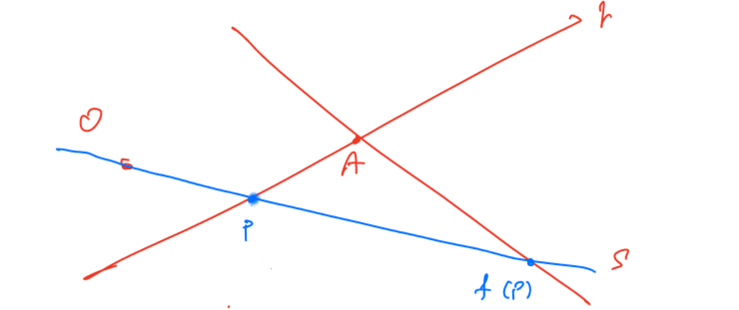
\includegraphics[scale=.6]{proiettivita.png}
\end{center}
$f$ è un isomorfismo proiettivo. La notazione si generalizza a $\pro^n$ nel modo seguente.\\
$S_1,S_2$ sottospazi di dimensione $k$, $H$ sottospazio tale che \[
H\cap S_1 = G\cap S_2 = \emptyset
.\] 
\[
\dim H = n  - k - 1
.\] Allora la restrizione a $S_1$ della proiezione su $S_2$ di centro $H$ è un isomorfismo proiettivo $f: S_1 \rightarrow S_2 $ detto prospettività di centro $H$
\newpage
\begin{defi}
	Una curva algebrica in $\A^2(K)$ è una classe di proporzionalità di polinomi non costanti di  $\K[x,y]$. Se  $f(x,y)$ è un rappresentante della classe, l'equazione 
	\[
	f(x,y) = 0
	.\] si dice equazione della curva
	\[
		 l= \{\icol{x\\y}\in \A^2|f(x,y) = 0\}
	.\] è il supporto della curva\\
	$\deg f$ grado della curva
\end{defi}
\textbf{Caso affine}\\
Sia $T: \A^2 \rightarrow \A^2$ l'affinità $T(X) = AX + C$
 \[
	 A = (a_{ij})\in GL(2,\L) \ \ C = \matrice{c_1\\c_2}
.\] 
Sia $l$ una curva di equazioni $f(x,y) = 0$
La curva $D$ di equazione 
\[
g(x,y) =0 
.\] 
ove $g(x,y) = f(a_{11}x_1+a_{12}y+c_1,a_{21}x+a_{22}y+c_2)$ \\
è detta la trasformata di $l$ tramite $T^{-1}$
 \[
 D = T^{-1}(l)
.\] 
Se $T^{-1}X = BX + d$ \ \ $(B = A^{-1}, \ \ldots)$\\
allora  $g(b_{11}x + b_{12}y + d_1, b_{21}x+b_{22}y + d_2) = A(x,y)$
quindi $l = T(D)$\\
è chiaro che se  $p(x,y)\in D$ allora $T(p)\in l$ e viceversa.\\
quindi i supporti si dicono affinamente equivalente
\begin{defi}
	Data $l$ curva affine, una curva affine $D$  si dice affinamente equivalente a $l$ se esiste un'affinità $T$ tale che $l = T(D)$
\end{defi}
\end{document}

